\documentclass{exam}

\usepackage{titling}
\usepackage{amsmath}
\usepackage{amsfonts}
\usepackage{mathtools}
\usepackage{float}
\usepackage{tikz}
\usepackage{graphicx}
\usepackage{subfig}
\usepackage{minted}
\usepackage{inconsolata}
\usepackage{tikz}

\graphicspath{ {./src/output} }


\setlength{\droptitle}{-5em}   


\renewcommand{\questionlabel}{\textbf{~\thequestion)}}
\renewcommand{\thepartno}{\roman{partno}}
\DeclarePairedDelimiterX{\norm}[1]{\lVert}{\rVert}{#1}

\newcommand*{\horzbar}{\rule[.5ex]{2.5ex}{0.5pt}}

\newenvironment{shiftedflalign*}{%
    \start@align\tw@\st@rredtrue\m@ne
    \hskip\parindent
}{%
    \endalign
}



\title{Homework 2 - Group 076}
\author{Aprendizagem 2021/2022}
\date{}

\cfoot{\thepage}

\begin{document}
    \maketitle
    \begin{tikzpicture}[overlay, remember picture]
        \node[xshift=3.5cm,yshift=-2cm] at (current page.north west) {
\includegraphics[scale = 0.35]{logo_ist.jpeg}};
    \end{tikzpicture}
    \vspace{-3.5em}
    \section{Pen and Paper}
    \begin{questions}
        \item Applying the linear basis function $\phi(\textbf{x}) = (1, \norm{\textbf{x}}_2, \norm{\textbf{x}}_2^2, \norm{\textbf{x}}_2^3)$ (with $\norm{\textbf{x}}_2 = \sqrt{x_1^2 + x_2^2 + x_3^2}$) to each instance $\textbf{x}^{(i)}$ ($i \in \{1, ..., 8\}$) in the training set, we get a new design matrix:
        \begin{equation*}
            \boldsymbol{\Phi} = 
            \begin{bmatrix}
                \horzbar & (\phi(\textbf{x}^{(1)}))^T & \horzbar \\
                \horzbar & (\phi(\textbf{x}^{(2)}))^T & \horzbar \\
                         & \vdots    &                     \\
                \horzbar & (\phi(\textbf{x}^{(8)}))^T & \horzbar \\
            \end{bmatrix} =
            \begin{bmatrix}
                1.0 & 1.4142 & 2.0 & 2.8284 \\
                1.0 & 5.1962 & 27.0 & 140.2961 \\
                1.0 & 4.4721 & 20.0 & 89.4427 \\
                1.0 & 3.7417 & 14.0 & 52.3832 \\
                1.0 & 7.2801 & 53.0 & 385.8458 \\
                1.0 & 1.7321 & 3.0 & 5.1962 \\
                1.0 & 2.8284 & 8.0 & 22.6274 \\
                1.0 & 9.2195 & 85.0 & 783.6613 \\
            \end{bmatrix}
        \end{equation*}
        To learn the regression model, we must compute the weight vector $\textbf{w}$ that minimizes the Sum of Squares error between the outputs $\textbf{z} = 
            \begin{bmatrix}
                1 & 3 & 2 & 0 & 6 & 4 & 5 & 7
            \end{bmatrix}^T$ and predictions $\textbf{\^{z}} = \boldsymbol{\Phi} \textbf{w}$ (i.e., $\textbf{w} = (\boldsymbol{\Phi}^T\boldsymbol{\Phi})^{-1}\boldsymbol{\Phi}^T\textbf{z}$):
        \begin{align*}
            \boldsymbol{\Phi}^T\boldsymbol{\Phi} &= 
            \begin{bmatrix}
                8.0 & 35.8843 & 212.0 & 1482.2811 \\
                35.8843 & 212.0 & 1482.2811 & 11436.0 \\
                212.0 & 1482.2811 & 11436.0 & 93573.5164 \\
                1482.2811 & 11436.0 & 93573.5164 & 793976.0 \\
            \end{bmatrix} \\
            (\boldsymbol{\Phi}^T\boldsymbol{\Phi})^{-1} &= 
            \begin{bmatrix}
                8.1955 & -6.2313 & 1.3049 & -0.0793 \\
                -6.2313 & 5.0781 & -1.1044 & 0.0686 \\
                1.3049 & -1.1044 & 0.2472 & -0.0157 \\
                -0.0793 & 0.0686 & -0.0157 & 0.001 \\
            \end{bmatrix} \\
            (\boldsymbol{\Phi}^T\boldsymbol{\Phi})^{-1}\boldsymbol{\Phi}^T&=
            \begin{bmatrix}
                1.7686 & -0.0811 & -0.6694 & -1.0069 & 1.3794 & 0.9051 & -0.785 & -0.5107 \\
                -1.0644 & -0.0319 & 0.5312 & 0.904 & -1.307 & -0.3922 & 0.8501 & 0.5101 \\
                0.1933 & 0.0436 & -0.0907 & -0.1868 & 0.3232 & 0.0524 & -0.1954 & -0.1395 \\
                -0.0107 & -0.0043 & 0.0044 & 0.0109 & -0.0214 & -0.0022 & 0.0123 & 0.011 \\               
            \end{bmatrix} \\
            \textbf{w} = (\boldsymbol{\Phi}^T\boldsymbol{\Phi})^{-1}\boldsymbol{\Phi}^T\textbf{z} &= 
            \begin{bmatrix}
                4.5835 & -1.6872 & 0.3377 & -0.0133
            \end{bmatrix} ^T
        \end{align*}
        \item Similarly to the previous question, we compute the image of each instance $\textbf{x}^{(i)}$ ($i \in \{1,2\}$) from the testing set by $\phi$ and place it in each row of the matrix $\boldsymbol{\Phi}$. Using the obtained weight vector $\textbf{w}$, we have the following estimates vector:
        \begin{equation*}
            \textbf{\^{z}} = \boldsymbol{\Phi}\textbf{w} = 
            \begin{bmatrix}
                1.0 & 2.0 & 4.0 & 8.0 \\
                1.0 & 2.4495 & 6.0 & 14.6969 \\
            \end{bmatrix}
            \begin{bmatrix}
                4.5835 \\
                -1.6872 \\
                0.3377 \\ 
                -0.0133 \\
            \end{bmatrix} = 
            \begin{bmatrix}
                2.4536 \\
                2.2816 \\
            \end{bmatrix}
        \end{equation*}
        Computing the root mean square error, we have:
        \begin{equation*}
           \mathrm{RMSE}(\textbf{\^{z}}, \textbf{z}) = \sqrt{\frac{1}{2}\sum_{i = 1}^{2}(\hat{z}_i - z_i)^2} = 1.2567
        \end{equation*}
        
        \item To make an equal depth binarization of $y_3$, we compute the median of the values of $y_3$ of all the instances in the dataset:
        \begin{equation*}
             \text{median}(\{y^{(i)}_{3}\}_{i = 1}^{10}) = 2.5
        \end{equation*}
        and make the following transformation to $y_3$:
        \begin{equation*}
            y_3 :=
            \begin{cases}
                0, & \text{if } y_3 < \text{median} \\
                1, & \text{otherwise}
            \end{cases}
        \end{equation*}
        Considering the given class targets, we have the following (training) data table:
        \begin{table}[H]
            \centering
            \begin{tabular}{llll}
            $y_1$ & $y_2$ & $y_3$ & $t$ \\ \hline
            1     & 1     & 0     & N   \\
            1     & 1     & 1     & N   \\
            0     & 2     & 1     & N   \\
            1     & 2     & 1     & N   \\
            2     & 0     & 1     & P   \\
            1     & 1     & 0     & P   \\
            2     & 0     & 0     & P   \\
            0     & 2     & 1     & P  
            \end{tabular}
        \end{table}
        \begin{itemize}
            \item Starting entropy:
            \begin{equation*}
                H(t) = - \sum_{i = 0}^{1}\frac{\#\{k|t^{(k)} = i\}}{8} \log_2\left(\frac{\#\{k|t^{(k)} = i\}}{8}\right) = - \left(\frac{1}{2}\log_2\left(\frac{1}{2}\right) + \frac{1}{2}\log_2\left(\frac{1}{2}\right)\right) = 1 \medspace bit
            \end{equation*}
            \item Variable conditional entropies and corresponding information gains ($\text{IG}(y_i) = H(t) - H(t|y_i))$:
            \begin{align*}
                H(t|y_1) &= \sum_{i = 0}^{2} \frac{\#\{k|y_1^{(k)} = i\}}{8}H(t|y_1 = i)\\
                &= - \sum_{i = 0}^{2} \frac{\#\{k|y_1^{(k)} = i\}}{8} \sum_{j = 0}^{1} \frac{\#\{k|y_1^{(k)} = i, t^{(k)} = j\}}{\#\{k|y_1^{(k)} = i\}} \log_2\left( \frac{\#\{k|y_1^{(k)} = i, t^{(k)} = j\}}{\#\{k|y_1^{(k)} = i\}}\right) \\
                &= - \frac{1}{4}\left( \frac{1}{2}\log_2\left(\frac{1}{2}\right) + \frac{1}{2}\log_2\left(\frac{1}{2}\right)\right) - \frac{1}{2} \left( \frac{3}{4}\log_2\left(\frac{3}{4}\right) + \frac{1}{4}\log_2\left(\frac{1}{4}\right)\right) - \frac{1}{4} \left( 0\log_2\left(0\right) + 1\log_2(1)\right) \\
                &= 0.65556  \text{ }bit\\
                H(t|y_2) &= - \frac{1}{4}\left(0\log_2(0) + 1\log_2(1)\right) - \frac{3}{8} \left( \frac{2}{3}\log_2\left(\frac{2}{3}\right) + \frac{1}{3}\log_2\left(\frac{1}{3}\right)\right) - \frac{3}{8} \left( \frac{2}{3}\log_2\left(\frac{2}{3}\right) + \frac{1}{3}\log_2\left(\frac{1}{3}\right)\right) \\
                &= 0.68872  \text{ }bit\\
                H(t|y_3) &= - \frac{3}{8}\left(\frac{1}{3}\log_2\left(\frac{1}{3}\right) + \frac{2}{3}\log_2\left(\frac{2}{3}\right)\right) - \frac{5}{8} \left( \frac{3}{5}\log_2\left(\frac{3}{5}\right) + \frac{2}{5}\log_2\left(\frac{2}{5}\right)\right) = 0.95121 \text{ }bit
            \end{align*}
            \begin{alignat*}{2}
                \text{IG}(y_1) = 1 - 0.65556  = 0.34436 \text{ }bit \quad & \text{IG}(y_2) = 0.31128 \text{ }bit \quad & \text{IG}(y_3) = 0.04879 \text{ }bit
            \end{alignat*}
        \end{itemize}
        Since $y_1$ yields the biggest information gain, it will take part in the first node in the decision tree and the following division in the dataset is obtained:
        \begin{table}[H]
            \centering
            \begin{tabular}{lll|lll|lll}
            \multicolumn{3}{c|}{$y_1  = 0$} & \multicolumn{3}{c|}{$y_1 = 1$} & \multicolumn{3}{c}{$y_1 = 2$} \\ \hline
            $y_2$     & $y_3$     & $t$    & $y_2$     & $y_3$     & $t$    & $y_2$     & $y_3$     & $t$    \\ \hline
            2         & 1         & N      & 1         & 0         & N      & 0         & 1         & P      \\
            2         & 1         & P      & 1         & 1         & N      & 0         & 0         & P      \\
                        &           &        & 2         & 1         & N      &           &           &        \\
                        &           &        & 1         & 0         & P      &           &           &       
            \end{tabular}
        \end{table}
        Partition $(y_1 = 2)$ has no uncertainty and we cannot reduce uncertainty in partition $(y_1 = 0)$ (note that there is only one value of $y_2$ (resp., $y_3$), so $H(t|y_2, y_1 = 1) = H(t|y_1 = 1)$ (resp., $H(t|y_3, y_1 = 1) = H(t|y_1 = 1)$), and there is no possible information gain). We thus proceed to divide partition $(y_1 = 1)$ even further in an analogous way as before: 
        \begin{itemize}
            \item Starting entropy:
        \end{itemize}
        \vspace{-1.75em}
        \begin{flalign*}
            H(t|y_1 = 1) &= - \sum_{i=0}^{1}\frac{\#\{k|t^{(k)} = i \wedge y_1^{(k)} = 1\}}{\#\{k|y_1^{(k)} = 1\}} \log_2\left(\frac{\#\{k|t^{(k)} = i \wedge y_1^{(k)} = 1\}}{\#\{k|y_1^{(k)} = 1\}}\right) \\
            &= - \left(\frac{3}{4}\log_2\left(\frac{3}{4}\right) + \frac{1}{4}\log_2\left(\frac{1}{4}\right)\right) = 0.81127 \medspace bit
        \end{flalign*}
        \vspace{-1.5em}
        \begin{itemize}
            \item Variable conditional entropies and corresponding information gains (where $\text{IG}(y_i|y_1 = 1) = H(t|y_1 = 1) - H(t|y_i, y_1 = 1)$; also note that $\#\{k|y_2^{(k)} = 0 \wedge y_1^{(k)} = 1\} = 0$, so $H(t|y_2 = 0, y_1 = 1)$ is not defined and we discard that term from the first sum):
        \end{itemize}
        \vspace{-1em}
        \begin{gather*}
            H(t|y_2, y_1 = 1) = \sum_{i = 1}^{2} \frac{\#\{k|y_2^{(k)} = i \wedge y_1^{(k)} = 1\}}{\#\{k|y_1^{(k)} = 1)\}}H(t|y_2 = i, y_1 = 1) \\
                = - \sum_{i = 1}^{2}  \frac{\#\{k|y_2^{(k)} = i \wedge y_1^{(k)} = 1)\}}{\#\{k|y_1^{(k)} = 1\}} \sum_{j = 0}^{1}  \frac{\#\{k|t^{(k)} = j \wedge y_2^{(k)} = i \wedge y_1^{(k) } = 1)\}}{\#\{k|y_2^{(k)} = i \wedge y_1^{(k)} = 1\}} \log_2\left(\frac{\#\{k|t^{(k)} = j \wedge y_2^{(k)} = i \wedge y_1^{(k) } = 1)\}}{\#\{k|y_2^{(k)} = i \wedge y_1^{(k)} = 1\}}\right) \\
                = - \frac{3}{4}\left( \frac{2}{3}\log_2\left(\frac{2}{3}\right) + \frac{1}{3}\log_2\left(\frac{1}{3}\right)\right) - \frac{1}{4} \left( 1\log_2(1) + 0\log_2(0)\right) 
                = 0.688721 \medspace bit\\
            H(t|y_3, y_1 = 1)
                = - \frac{1}{2}\left( \frac{1}{2}\log_2\left(\frac{1}{2}\right) + \frac{1}{2}\log_2\left(\frac{1}{2}\right)\right)
                =  0.5 \medspace bit
        \end{gather*}
        \vspace{-1.5em}
        \begin{alignat*}{2}
            \text{IG}(y_2|y_1 = 1) = 0.81127 - 0.688721  = 0.1225979 \text{ }bit \quad & \text{IG}(y_3|y_1 = 1) = 0.81127 - 0.5  = 0.31127 \text{ }bit 
        \end{alignat*}
        As $y_3$ provides the biggest information gain, it will divide the partition $(y_1 = 1)$. The resulting dataset cannot be further partitioned ($(y_1 = 1, y_3 = 1)$ has no uncertainty and we can't obtain information gain from dividing $(y_1 = 1, y_3 = 0)$ for the same argument as the one applied to $(y_1 = 0)$):
        \begin{table}[H]
            \centering
            \begin{tabular}{lll|ll|ll|lll}
            \multicolumn{3}{c|}{$y_1  = 0$} & \multicolumn{4}{c|}{$y_1 = 1$}                                  & \multicolumn{3}{c}{$y_1 = 2$} \\ \hline
            $y_2$     & $y_3$     & $t$     & \multicolumn{2}{l|}{$y_3 = 0$} & \multicolumn{2}{l|}{$y_3 = 1$} & $y_2$     & $y_3$     & $t$    \\ \hline
            2         & 1         & N       & $y_2$           & $t$          & $y_2$           & $t$          & 0         & 1         & P      \\ \cline{4-7}
            2         & 1         & P       & 1               & N            & 1               & N            & 0         & 0         & P      \\
                      &           &         & 1               & P            & 2               & N            &           &           &       
            \end{tabular}
        \end{table}
        Thus, we have the desired decision tree:
        \vspace{-0.25em}
        \begin{table}[H]
            \centering
            \begin{tabular}{llccrr}
            \multicolumn{2}{r}{$y_1 = 0$}  & \multicolumn{2}{c}{$y_1 = 1$}    & \multicolumn{2}{l}{$y_1 = 2$}  \\
            \multicolumn{2}{c}{$\swarrow$} & \multicolumn{2}{c}{$\downarrow$} & \multicolumn{2}{c}{$\searrow$} \\
            N/P         &                  & $y_3 = 0$       & $y_3 = 1$      &                     & P        \\
                        &        & $\downarrow$    & $\downarrow$   &        &          \\
                        &                  & N/P             & N              &                     &         
            \end{tabular}
        \end{table}
        \item Considering the computed decision tree, for $\textbf{x}^{(9)} = 
        \begin{bmatrix}
            2 & 0 & 0
        \end{bmatrix}^T$ 
        we have that $\textbf{\^{t}}(\textbf{x}^{(9)}) = \text{P}$, and, for $\textbf{x}^{(10)} = 
        \begin{bmatrix}
            1 & 2 & 1
        \end{bmatrix}^T$, we have that $\textbf{\^{t}}(\textbf{x}^{(10)}) = \text{N}$. Since $\textbf{t}(\textbf{x}^{(9)}) = \text{N}$ and $\textbf{t}(\textbf{x}^{(10)}) = \text{P}$, there are no true positives and no true negatives in the classification of these instances. Hence, accuracy on the testing data is 0 according to the following formula: $\text{Accuracy} = \frac{TP + TN}{P + N}$.

    \end{questions}
    \section{Programming and critical analysis}
    \begin{questions}
        \setcounter{question}{4}
        \item
        \begin{parts}
            \item { \quad}
            \vspace{-3.0em}
            \begin{figure}[H]
                \centering
                {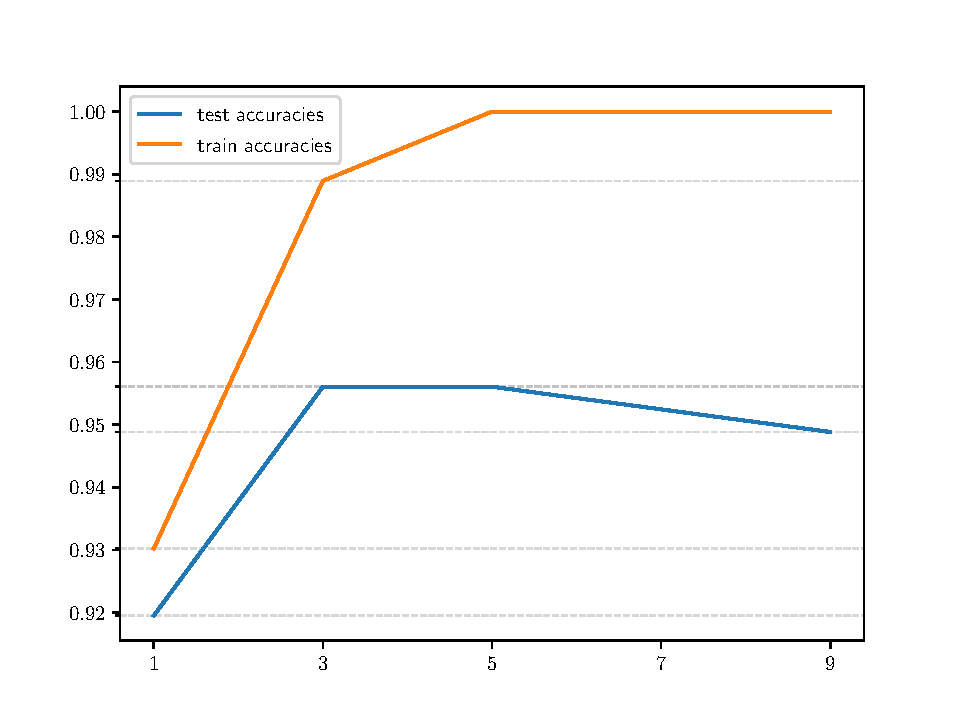
\includegraphics[scale = 0.60]{accuracy_n_features.pdf} }
            \end{figure}
            \item  {\quad}
            \vspace{-3.0em}
            \begin{figure}[H]
                \centering
                {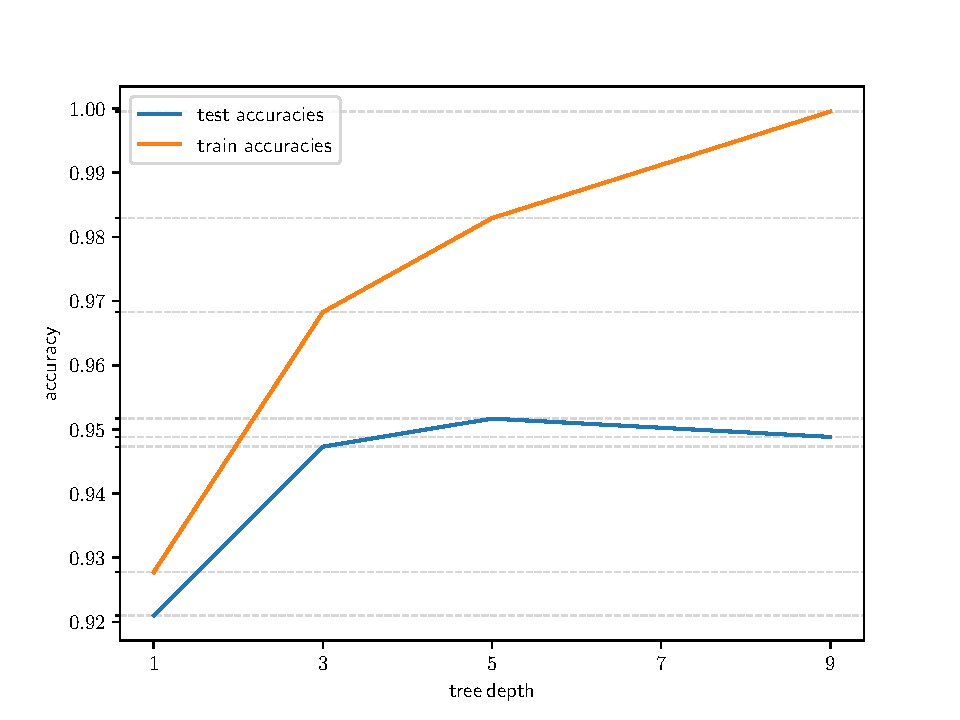
\includegraphics[scale = 0.60]{accuracy_n_tree_depths.pdf} }
            \end{figure}
        \end{parts}
        %\item Both plots exhibit the following correlation: %with the increase of tree size (by number of relevant %features or depth), training accuracy rises but %testing accuracy starts to fall after a certain point, %thus revealing a tendency of overfitting to the %training data. These behaviours can be explained by %the following reasons:
        \item The correlation between tendencies shown by both plots is due to the following reasons:
        \vspace{-0.4em}
        \begin{itemize}
            \item depth and number of considered features are positively correlated: if there are more features then it is expected that rules consider a bigger number of said features, making the decision tree deeper; if we loosen the depth threshold, then there are less restriction on how many features to consider. Therefore, the interaction between depth/no. of features and training/testing accuracy can become highly similar;
            \item both an increased number of considered features and tree depth make splits more granular and the rules more specific to the regularities of the training data, making it harder for the model to generalize to unseen data data (i.e., overfitting). Hence the always-rising tendency in training accuracy and a decay in testing accuracy from a certain tree depth/no. of features onwards.
            %\item considering features that are not very %relevant to classification (according to mutual %information) can originate rules that are too %specific to regularities of the training data, %making it harder for the tree to generalize to %unseen data. 
            %\item loosening the tree depth threshold can cause %an excessive split granularity (and thus the %formation of meaningless rules that consider more %factors than needed). 
        \end{itemize}
        \item According to the plot in question 5) (ii), the most suitable tree depth is 5, since it is the one that maximizes mean testing accuracy across train/test folds. Consequently, it is the one that is less expected to overfit, following the last argument in the previous question. 
    \end{questions}
    \pagebreak
    \section{Appendix}
    \inputminted{python}{src/ex02.py}
    
    
\end{document}